\documentclass[border=1cm,10pt]{standalone}

% I only need the arrows for this one.
\usepackage{tikz}
\usetikzlibrary{arrows}
\usetikzlibrary{decorations.pathmorphing}
\usetikzlibrary{decorations.markings}
\usetikzlibrary{trees}

\begin{document}

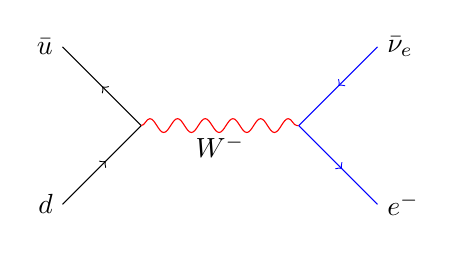
\begin{tikzpicture}[
  boson/.style={decorate, decoration={snake}, draw=red},
  lepton/.style={draw=blue, postaction={decorate},
        decoration={markings,mark=at position .55 with {\arrow[draw=blue]{>}}}},
  alepton/.style={draw=blue, postaction={decorate},
        decoration={markings,mark=at position .55 with {\arrow[draw=blue]{<}}}},
  quark/.style={draw=black, postaction={decorate},
        decoration={markings,mark=at position .55 with {\arrow[draw=black]{>}}}},
  aquark/.style={draw=black, postaction={decorate},
        decoration={markings,mark=at position .55 with {\arrow[draw=black]{<}}}},
]

% Draw the quarks
\draw[aquark] (0,2) node[left] {$\bar{u}$} -- (1,1) ;
\draw[quark] (0,0) node[left] {$d$} -- (1,1) ;

% Draw the boson
\draw[boson] (1,1) -- (3,1) node[midway,below] {$W^{-}$} ;

% Draw the lepton and neutrino
\draw[lepton] (3,1) -- (4,0) node[right] {$e^{-}$} ;
\draw[alepton] (3,1) -- (4,2) node[right] {$\bar{\nu}_e$} ;

% u + bar d → W+ → e+ nue

\end{tikzpicture}

\end{document} 
